\section{Image Features}

Image features are about detecting the location of patterns in images, e.g. edge detection or facial landmarks.


\subsection{Template Matching}

Given an template $t$, e.g. template describing an eye, we want to locate an area, in an image $s$, that best fits this template. Alternatively we could also look for areas that match this template by a certain threshold. \medskip

To search for the best match, we try to minimize the mean squared error. This is the same as maximizing the area correlation:
$$r(p, q) = \sum_{x = -\infty}^\infty \sum_{y = -\infty}^\infty s(x,y) \cdot t(x - p, y - q) = s(p,q) * t(-p, -q)$$


\subsection{Edge Detection}

We have previously seen kernels that can detect horizontal edges. To expand on this, we differentiate the following kernels:
$$ \text{Prewitt} 
\begin{bmatrix}
    -1 & 0 & 1\\
    -1 & 0 & 1\\
    -1 & 0 & 1
\end{bmatrix}
\qquad
\text{Sobel} 
\begin{bmatrix}
    -1 & 0 & 1\\
    -2 & 0 & 2\\
    -1 & 0 & 1
\end{bmatrix}
$$

We can also transpose these kernels to detect horizontal edges. From the resulting images (horizontal / vertical edges) we take the log sum squared and use different thresholds to achieve the final result.
\begin{center}
	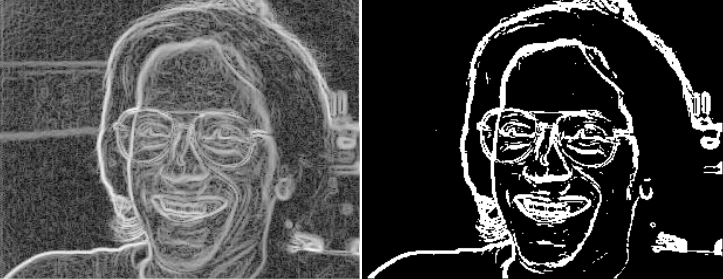
\includegraphics[width=\linewidth]{edge_detection.png}
\end{center}

\subsubsection{Laplacian Operator}

The idea behind the Laplacian operator is to detect discontinuities in the second derivative. This corresponds to detecting zero-crossings. The operator is isotropic (rotationally invariant) and can be implemented with one of the following kernels:
$$
\begin{bmatrix}
    0 & 1 & 0\\
    1 & -4 & 1\\
    0 & 1 & 0
\end{bmatrix}
\quad
\text{ or }
\quad
\begin{bmatrix}
    1 & 1 & 1\\
    1 & -8 & 1\\
    1 & 1 & 1
\end{bmatrix}
$$

This operator is very sensitive to fine details and noise, therefore we might need to blur the image first. Additionally it will respond equally to weak and strong edges, so we want to suppress edges with low gradient magnitude. Blurring and applying the Laplacian operator can be combined into a convolution with Laplacian of Gaussian (LoG). Combining LoG with gradient based threshold delivers the best result.
\begin{center}
	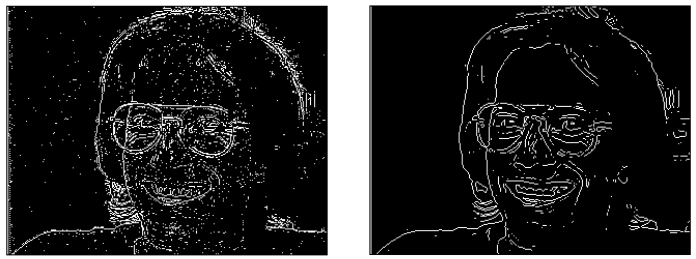
\includegraphics[width=\linewidth]{log_edge_detection.png}
\end{center}

\subsubsection{Canny Edge Detector}

The Canny edge detector works by first smoothing the image with a Gaussian filter. Then we compute the gradient magnitude (Sobel, Prewitt, ...) and the angle of the gradient. After this we want to apply non-maxima suppression to the gradient magnitude image. Combining this with double thresholding, to detect strong and weak edge pixels, and rejecting weak edge pixels not connected with strong edge pixels, results in the Canny edge detector.
\begin{center}
	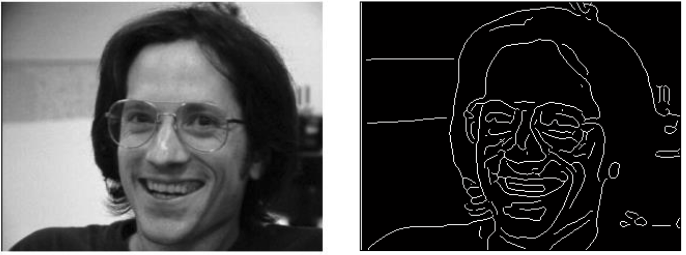
\includegraphics[width=\linewidth]{canny_edge_detection.png}
\end{center}


\subsection{Hough Transform}

Hough transform can be used to find higher order entities in an image, e.g. lines or circles. The Hough transform is a generalized template matching technique. Considering detection of straight lines (y = mx + c), for each edge pixel there are infinitely many possible lines. We plot these possible lines in the 2D space formed by its parameters, we end up with a single line.
\begin{center}
	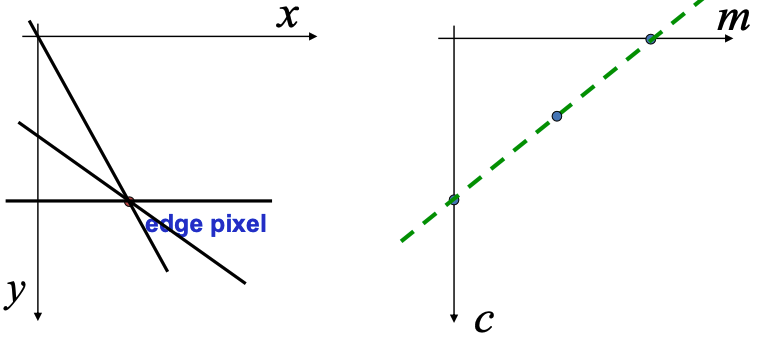
\includegraphics[width=\linewidth]{hough_transform.png}
\end{center}

If we do this for multiple edge points and subdivide the parameter space into discrete bins, we can find the bin with the most possible lines. This gives us the detected line.
\begin{center}
	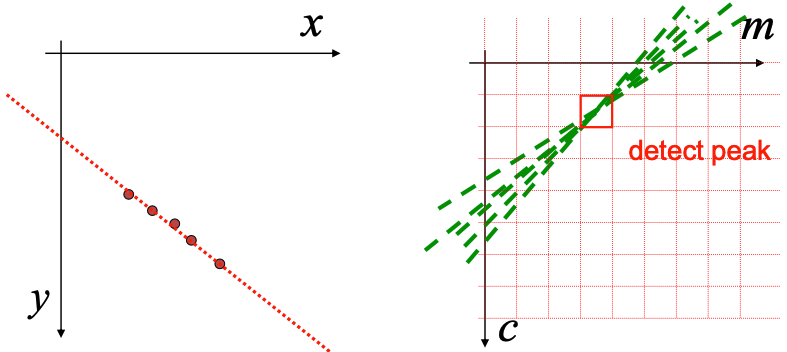
\includegraphics[width=\linewidth]{hough_transform2.png}
\end{center}

There is a problem with this approach, the parameter space is infinite. To avoid this problem we choose an alternative parametrization, in this case we represent a line as an angle and the distance from the origin. Now the representations in parameter space are not lines but sine waves. Again we find the maxima to find our lines.
\begin{center}
	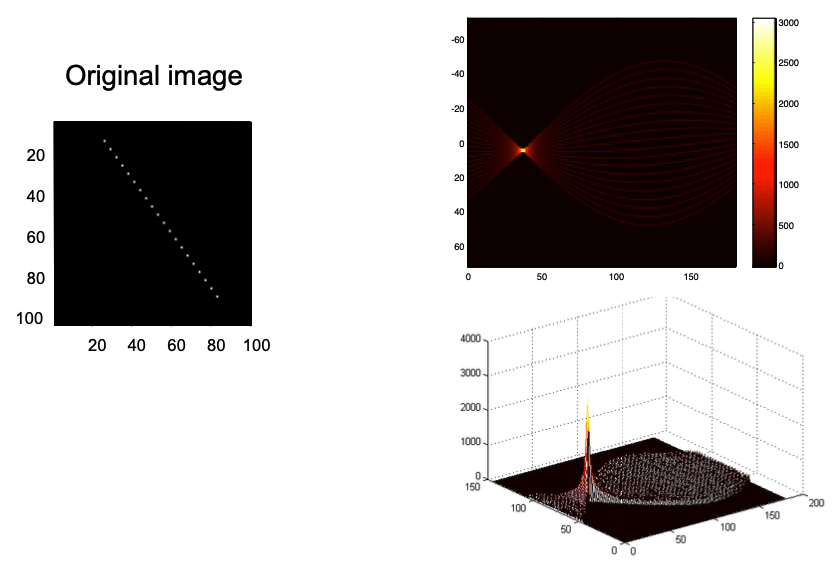
\includegraphics[width=\linewidth]{hough_transform3.png}
\end{center}

To find multiple lines we do non-maxima suppression and keep every strong peek. To expand this concept to circle detection we simply change the parameter space.


\subsection{Keypoint Detection}

We might want to only find corners and not edges. We want this corner localization to be accurate, invariant and robust. We define the following:
$$\textbf M = \left( \sum_{(x,y) \in \text{window}} 
\begin{bmatrix}
    f_x^2(x,y) & f_x(x,y) f_y(x,y) \\
    f_x(x,y) f_y(x,y) & f_y^2(x,y)
\end{bmatrix}
\right)$$

$$S(\Delta x, \Delta y) = (\Delta x, \Delta y) \textbf{ M } (\Delta x, \Delta y)^\top$$

Hereby $f_x$ is the horizontal gradient and $f_y$ the vertical gradient. $\textbf{M}$ is called the structure matrix or nomal matrix. To detect feature points we know try to find points for which $\min \Delta^\top \textbf M \Delta, || \Delta || = 1 $ is large. This is the same as maximizing the eigenvalues of $\textbf M$. The eigenvalue allow us to define a measure of "cornerness" (smaller $k$ means more strict):
$$C(x,y) = \det \textbf M - k \cdot (\text{trace } \textbf M)^2 = \lambda_1 \lambda_2 - k \cdot (\lambda_1 + \lambda_2)^2$$

If we plot the values for the eigenvalues, we can divide the space as follows:
\begin{center}
	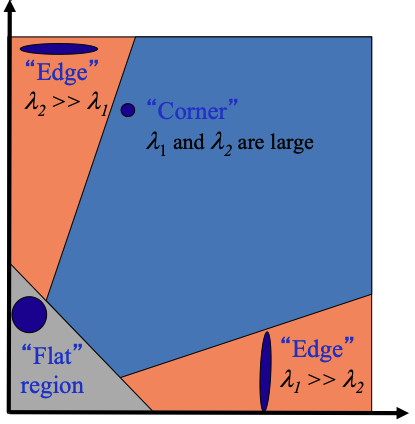
\includegraphics[width=0.6\linewidth]{keypoint_detection.png}
\end{center}

One problem of this approach is that it is not invariant to scale. \medskip

To compare different images, e.g. for combining images. We use thresholded image gradients that are sampled over an array of locations in scale space. This can then be used for example to stich images together (SIFT).






